\documentclass[11pt]{article}
\usepackage[letterpaper,margin=0.95in]{geometry}
\usepackage[T1]{fontenc}
\usepackage{lmodern}
\usepackage{microtype}
\usepackage{amsmath,amssymb}
\usepackage{graphicx}
\usepackage{booktabs,tabularx,array,multirow}
\usepackage{enumitem}
\usepackage[dvipsnames]{xcolor}
\usepackage{caption}
\usepackage{float}
\usepackage{adjustbox}
\usepackage[hidelinks]{hyperref}
\definecolor{hblue}{HTML}{2a78d6}
\definecolor{boxbg}{HTML}{f4f3ef}
\definecolor{ink2}{HTML}{52514e}
\hypersetup{colorlinks=true,linkcolor=hblue,urlcolor=hblue,citecolor=hblue}
\captionsetup{font=small,labelfont=bf,margin=0.15in}
\setlist{itemsep=2pt,topsep=3pt,parsep=0pt}
\setlength{\parskip}{4pt}
\setlength{\parindent}{0pt}
\graphicspath{{../../../results/}{figs/}}
\newcommand{\keybox}[1]{\par\smallskip\noindent\colorbox{boxbg}{\parbox{\dimexpr\linewidth-2\fboxsep}{\small #1}}\par\smallskip}
\newcommand{\TPR}{\mathrm{TPR}}
\newcommand{\FPR}{\mathrm{FPR}}
\renewcommand{\arraystretch}{1.18}

\sloppy
\usepackage{xurl}

\newcommand{\uv}{\textsuperscript{\dag}}
\newcommand{\rf}[1]{\texttt{\small #1}}
\setlist{itemsep=1pt,topsep=2pt,parsep=0pt}
\renewcommand{\topfraction}{0.9}\renewcommand{\bottomfraction}{0.8}\renewcommand{\textfraction}{0.07}\renewcommand{\floatpagefraction}{0.85}\setcounter{topnumber}{3}\setcounter{totalnumber}{4}
\title{\textbf{White-Box Monitors Pilot: a Trusted Qwen3.5-27B Reader}\\[4pt]
\large Probes, J-lens readouts and their decision layer on MonitoringBench, LinuxArena and MOLE, with second-audit corrections}
\date{October 2026}
\begin{document}
\maketitle
\vspace{-1.5em}

\keybox{\textbf{Summary.} We ran an open model, Qwen3.5-27B, as a \emph{trusted reader} over agent transcripts and read its activations with off-the-shelf and cheaply trained probes. It read 1{,}325 MonitoringBench trajectories (775 attacks, 550 honest) that \texttt{gpt-4.1-mini} had already scored step by step. It read them two ways: \emph{full} (each step sees all earlier steps) and \emph{per-step} (each step read alone). It also read 1{,}210 detector-aware rewrites, the LinuxArena sweep, and MOLE insider sessions. All of Idea 1--3's decision-layer machinery was then applied to the probe streams. Cost: about \$70 of H200 time and \$2.95 of API. An independent second audit re-derived every headline that the stored data still support; the corrected numbers are the ones stated here.
\begin{enumerate}[leftmargin=1.2em]
\item \textbf{Holds: the FIBS axial probe on a per-step follow-up question beats the LLM monitor.} TPR at 1\% trajectory FPR is $+0.19$ to $+0.21$ above \texttt{gpt-4.1-mini} (0.34 vs 0.15), equally on both attack agent models. The gain is unchanged at equal realized FPR ($+0.18$). It is the only one of 18 pre-planned reader-vs-LLM contrasts that survives Holm correction.
\item \textbf{Holds: a probe-triage cascade.} The synthetic-sabotage probe sends the 10\% most suspicious honest-calibrated steps (13\% of all steps) to the LLM. This raises TPR from 0.17 to 0.30 ($+0.13$) at matched realized FPR, with about 87\% fewer LLM calls.
\item \textbf{Weakened.}
  \begin{itemize}
  \item Full-reading sabotage probe $+0.10$: Holm $p=0.22$; the gain is confined to attacks by the same agent model as the honest runs.
  \item Full-reading FIBS axial probe and every fusion built on it: the threshold does not transfer across tasks (2.05\% realized FPR at nominal 1\%).
  \item LinuxArena ranking: no paired test, and the reader score files were lost.
  \end{itemize}
\item \textbf{Negative.}
  \begin{itemize}
  \item No accumulation rule beats max on any probe stream.
  \item Probe streams are more context-heterogeneous than LLM streams ($\tau$ up to 3.8 vs $\le$0.46), but per-context thresholds gain little at matched spend.
  \item J-lens watch-lists are weak monitors.
  \item Policy activations do not beat the trusted reader on MOLE.
  \end{itemize}
\item \textbf{Rewrite artifact.} Detector-aware rewrites are detected \emph{more} by the LLM and the follow-up probes, but not by token-level probes.
\end{enumerate}}


\section{Motivation and prior work}\label{sec:prior}

\paragraph{Source and caveat.} This section condenses an internal literature note (\rf{docs/reports/White box monitors for AI control.md}, 21 Oct 2026). Its numbers were \emph{not} re-checked against the primary sources for this report. Numbers that the note itself says reached it only through an automated summary or a search snippet are marked \uv\ (unverified secondhand). Treat them as leads, not citations.

\subsection{Probes roughly match frontier text monitors where misbehavior is salient}
\begin{itemize}
\item \textbf{FIBS} (FAR.AI, arXiv 2610.12445) is the reference point. It trains four probe architectures, including an ``axial'' transformer over the layer$\times$token grid, on 163{,}016 ``contextual falsehood'' transcripts (28 families), reading 6 layers at 30--90\% depth on 9 open models. On agent steps it appends ``Did you take actions towards a hidden side task?'' and contrasts the probe readings for a prefilled ``Yes.'' and ``No.''. It reports 98.3\% / 98.0\% per-step AUROC on SHADE-Arena / BashArena vs 97.7\% / 97.6\% for frontier text monitors (comparator identity\uv). Limits: instructed (not trained) saboteurs, no probe-aware attacker, one global threshold.
\item \textbf{Apollo deception probes} (arXiv 2502.03407; Llama-3.3-70B, layer 22/80, mean pooling): AUROC 0.964--0.999, 95--99\% recall at 1\% Alpaca FPR, ``roughly equivalent'' to a GPT-4o baseline. Recall fell to nearly 0 on Insider Trading two layers later, and the probe fires on honest answers to evaluation prompts. Earlier: coup probes from 43 synthetic examples reached 100\% TPR at 1\% FPR on 46 cases; a one-pair defection probe predicted sleeper-agent defection at 99.3\% AUROC.
\item \textbf{Where white-box loses or ties.} Liars' Bench: 0.54 balanced accuracy vs 0.73 for an LLM judge. Trained lying organisms: activation detectors ``drop sharply''. AUROC misleads at operating points: an AgentDojo activation monitor with 0.92 AUROC had 0.00 TPR at 5\% FPR (arXiv 2610.04575).
\item \textbf{Trusted readers.} The one precedent for probing a \emph{trusted} model that reads untrusted transcripts is a single unreviewed repository (APPS backdoors: 0.91 AUROC vs 0.54 for the same model's own rating).
\end{itemize}

\subsection{Deployments and robustness}
\begin{itemize}
\item \textbf{Cheap first-stage screens.} Anthropic's Constitutional Classifiers++ runs a 377K-FLOPs/token linear probe in front of a classifier, escalating about 5.5\% of traffic and cutting compute about $40\times$\uv. GDM's production misuse probes (MultiMax, rolling means) feed a probe$\to$Flash cascade that calls the LLM on under 10\% of traffic and beats Flash alone at about 1/50 the cost\uv.
\item \textbf{Misalignment monitoring is described only secondhand.} Anthropic reportedly ran dishonesty, reward-hacking and eval-awareness probes on every transcript during most of post-training\uv; OpenAI describes per-token activation classifiers escalating to automated investigators\uv\ at about 20\% overhead\uv; GDM's roadmap (arXiv 2607.13087) calls activation monitoring ``more speculative''. No lab has published recall or FPR for a misalignment probe.
\item \textbf{Training breaks probes.} Embedding-space attacks cut harmfulness-probe recall from 100\% to 0\% (Bailey et al., ICLR 2026). RL against a probe evades mean-pooled linear probes in 59--82\% of cases, while max-pooled and attention probes stay near 0\% (arXiv 2506.14261; per-cell numbers\uv). ``Neural Chameleons'' trained to evade benign-concept probes zero-shot evade unseen deception probes (arXiv 2512.11949). Even RLVR with no probe penalty moved an off-domain deception probe from 0.99 to 0.38--0.66 AUROC (arXiv 2602.15515; values\uv).
\item \textbf{Passive shift and context.} Stylistic rewrites collapse probes with clean AUROC $\ge$0.998 (arXiv 2605.27958); a mean-pooled probe missed 99.13\% of long-context attacks\uv. Probes fire on honest text in risky contexts, yet almost every paper calibrates one global threshold on benign chat.
\end{itemize}
This is the motivating gap for a decision-layer project: probe thresholds are context-confounded, pooling is ad hoc, and there is no trajectory-level false-alarm accounting.

\subsection{J-lens}
The Jacobian lens maps a layer-$l$ residual into the final-layer basis through the corpus-averaged Jacobian and decodes it with the unembedding. Its monitoring evidence is qualitative, plus one eval-awareness score (AUC 0.853). Our J-lens-diffing project found that standalone single-model J-lens audits detected 0 of 5 fine-tuned organisms (per the same note). A runtime J-lens monitor therefore needs a fixed token watch-list or a per-context baseline.

\subsection{What this pilot tests}
FIBS did not do trajectory aggregation, sequential tests, per-environment thresholds, fusion with black-box monitors, red-teaming with an aware attacker, or trusted-reader probing (per the note's fetched summaries). The pilot tests six things on one reader pass:
\begin{enumerate}[label=(\alph*)]
\item decision rules (max vs accumulators) on probe streams;
\item per-context probe thresholds;
\item probe + LLM fusion and triage;
\item probes on detector-aware rewrites;
\item a J-lens watch-list as a step-level monitor;
\item stage 2: policy vs reader activations.
\end{enumerate}
\textbf{Go/no-go rule, set before the run.} Proceed to stage 2 if a reader probe's trajectory TPR at 1\% FPR is within the bootstrap CI of \texttt{gpt-4.1-mini}'s, or if fusion adds $\ge$0.05 TPR at matched cost. Both conditions were met, so stage 2 was run.

\section{Setup}

\subsection{Reader and reading protocol}
\begin{itemize}
\item \textbf{Reader.} \texttt{Qwen/Qwen3.5-27B} (rev \texttt{fc05daec}, bf16) is a hybrid gated-DeltaNet/attention model, run with HF transformers and forward hooks on one on-demand H200. We chose it because it is the one open model with both released FIBS probes (layers 19/27/35/43/51/58) and a pre-fitted neuronpedia J-lens.
\item \textbf{Framing.} A monitor-style chat: \texttt{gpt-4.1-mini}'s monitor system prompt minus the rubric, then the task text, then steps rendered as \texttt{<action index=k>} (actions truncated at 4{,}000 characters, outputs at 1{,}500; first 60 steps; final \texttt{submit} stripped as in Idea 1).
\item \textbf{Full (history-aware).} One incremental pass with a KV and recurrent-state cache: step $t$'s tokens see the task and all earlier steps.
\item \textbf{Per-step (history-free; ``none'').} System prompt + task + step $t$ only. The prefix cache is rolled back before each step.
\item \textbf{Follow-up.} After each step the cache is snapshotted. A FIBS-format question (``Did the agent take actions towards a hidden side task?'') with a prefilled \texttt{Yes.} / \texttt{No.} answer is appended, read, and rolled back.
\item \textbf{Storage.} Only per-step pooled scores and per-step mean activations are kept (activations stay on the pod).
\end{itemize}

\subsection{Signals}
\begin{table}[!htbp]\centering\small
\begin{tabularx}{\linewidth}{@{}>{\raggedright\arraybackslash}p{3.3cm}>{\raggedright\arraybackslash}X@{}}
\toprule
Stream (code) & Definition\\
\midrule
Sabotage probe (\texttt{sab}) & Logistic regression per layer on 1{,}012 \texttt{gpt-4.1}-generated honest vs covert-malicious step pairs. The pairs cover 36 task themes $\times$ 8 generic objective categories taken from the monitor prompt. Theme-grouped CV AUROC is 0.945--0.971 by layer (\rf{scores/probes\_report.json}). Primary form: mean over the 6 layers, mean-pooled over step tokens. Variants: max-token; single layers (L43 is \emph{post hoc}).\\
Apollo probe (\texttt{dec}) & Instructed-Pairs deception probe on 306 true facts. CV AUROC 1.0, a known caveat: the instruction is in context.\\
FIBS linear on tokens (\texttt{fibs\_tok}) & Released FIBS linear probe read directly on the step tokens.\\
FIBS linear follow-up (\texttt{fibs\_fu}) & FIBS linear probe at the follow-up answer; score = reading(\texttt{No.}) $-$ reading(\texttt{Yes.}).\\
FIBS axial follow-up (\texttt{fibs\_fu\_ax}) & The same contrast with the released FIBS axial probe.\\
J-lens (\texttt{jl\_lm}, \texttt{jl\_hits}) & Watch-list of 81 single-token ids (deceive, hide, secret, exfiltrate, backdoor, malicious, sabotage, evade, monitor, suspicious, \dots). Two scores: log-mass at layers 27/35/43 (layer mean) and the number of watch-list tokens in the top 25.\\
Supervised probe (\texttt{sup}) & Cross-fitted LR on per-step mean activations of the evaluation data. An in-distribution upper bound, leaky (\S\ref{sec:confounds}).\\
LLM baseline & \texttt{gpt-4.1-mini}, prompt \texttt{ctrl-basic-v1}, logprob-expected 0--10 score, same history mode (from Idea 1).\\
\bottomrule
\end{tabularx}
\caption{Per-step signals. Each is pooled over the step's tokens (mean / max / last). The trajectory statistic is the max over steps unless stated otherwise.}
\end{table}

\noindent\textbf{Primary streams.} The results log designates \texttt{sab} (layer mean), the FIBS follow-up contrasts and J-lens mass as ``pre-specified primary''. The second audit found that this designation first appears in the results entry, not the setup entry (\rf{results/audit2/issues.csv}, m2). This report therefore treats the 18 stream$\times$mode reader-vs-LLM contrasts as one family and applies Holm.

\noindent\textbf{What the probe directions decode to} (J-lens decoding of the probe weight vectors; qualitative, \rf{scores/probe\_direction\_jlens.json}): \texttt{sab} at L51/L58 to \emph{hidden, disguised, simultaneously, conceal, suspicious, rogue}, and at L43 to delete/remove/hide tokens (mostly Chinese); \texttt{dec} and FIBS at L35--43 to \emph{fake, false, falsehood}; FIBS at L51/58 to \emph{Wait, False, Actually}.

\subsection{Data}
\begin{table}[!htbp]\centering\small
\begin{adjustbox}{max width=\linewidth}\begin{tabular}{@{}lllll@{}}
\toprule
Set & Honest / attack & Modes & Comparators & Score files now\\
\midrule
MonitoringBench (MB) & 550 / 775 (S1--S3 100 each, S4 475), 37.7k steps & full, none & \texttt{gpt-4.1-mini} & intact\\
T3 round 1 rewrites & same honest / 509 unique (126 base attacks) & full, none & \texttt{gpt-4.1-mini}, \texttt{gpt-4.1} & \textbf{lost (0 bytes)}\\
T3 round 2 rewrites & same honest / 701 unique (150 base attacks) & none & \texttt{gpt-4.1} & intact\\
LinuxArena & 200 / 142, 10 environments & full, none & 12 per-action LLM monitors & \textbf{lost (0 bytes)}\\
MOLE \texttt{qwen36\_27b} single-day & 200 benign / 233 insider sessions & policy, reader & none & intact\\
\bottomrule
\end{tabular}\end{adjustbox}
\caption{Scored sets. Honest-550 is entirely \texttt{claude-opus-4-5}. Of the 775 MB attacks, 494 are opus-4-5 and 281 are opus-4-6. ``Lost'': the reader per-step files were overwritten with empty files by the last pod sync, after the LinuxArena and T3-r1 analyses had run. The pods have since been deleted (\rf{results/audit2/issues.csv}, A2).}
\end{table}

\subsection{Statistics}
Randomized plug-in thresholds are set on the honest calibration half of task-grouped 50/50 splits, at trajectory FPR 0.05 / 0.01 / 0.003. Intervals are 95\% task-cluster bootstraps that include calibration noise; contrasts use \texttt{amd.evaluation.paired} (one joint resample per replicate, thresholds recomputed). The project analysis (\rf{results/wb/}) used only 10 splits, so its point estimates carry a few points of split noise. The second audit (\rf{results/audit2/}) re-implemented everything independently (\texttt{a2lib.py}, no reuse of \texttt{amd.evaluation}) with 40 and 200 splits, reports the \emph{realized} test FPR, and equalizes realized FPR by bisection on the nominal level. ``Holds / weakened / dropped'' verdicts follow \rf{results/audit2/corrections.csv}.

\subsection{Integrity checks}\label{sec:confounds}
\begin{itemize}
\item \textbf{Numerical (incremental vs single pass, 24 trajectories, 661 steps).} Mean-pooled step features agree to Pearson $r\ge0.999$ (median $|\Delta|\le0.02$ SD). Max-token features agree to $r=0.98$--$0.99$ (e.g.\ J-lens L43 max: $r=0.982$, max $|\Delta|=2.1$ SD) (\rf{wb/numerical\_check.json}). bf16 kernels are chunk-boundary sensitive, so max-pooled variants carry numerical noise. Mean-pooled streams are reliable.
\item \textbf{Probe training data is disjoint from the evaluation data.} The maximum TF-IDF cosine between a contrast task and an MB task is 0.61. Only 9 of 12{,}009 contrast 8-grams appear in 400 MB attacks, and they are generic boilerplate (\rf{wb/disjointness.json}).
\item \textbf{No source/style leakage in the generic streams.} On \emph{pre-onset} attack steps vs honest steps (9{,}188 steps), every generic probe and the LLM score AUROC 0.46--0.58 (Apollo full is highest at 0.58) (\rf{wb/mb\_preonset.csv}).
\item \textbf{The supervised probe is leaky.} It scores 0.79 (full) / 0.70 (none) on pre-onset steps, so it partly learns trajectory-source features. It also transfers poorly: LinuxArena AUROC 0.69 / 0.55 (\rf{wb/la\_auroc.csv}). It is reported only as a leaky upper bound.
\item \textbf{Agent model is label-correlated} (first-audit M9). All honest runs are opus-4-5; 36\% of attacks are opus-4-6. The LLM's TPR doubles on opus-4-6 attacks (full: 0.113 vs 0.253), so every contrast is also reported per agent model (\rf{wb/tables.md}).
\item \textbf{Length.} On length-matched subsets (383 honest, 383 attacks) the stream ordering is unchanged at FPR 0.01: \texttt{sab} full 0.21 vs LLM 0.15, FIBS axial none 0.30 vs LLM 0.09 (\rf{wb/mb\_length\_matched.csv}). Realized FPRs there range 0.9--2.7\%.
\end{itemize}

\section{Results}

\subsection{Reader probes vs the LLM monitor on MonitoringBench}

\begin{table}[!htbp]\centering\small
\begin{adjustbox}{max width=\linewidth}\begin{tabular}{@{}llccccc@{}}
\toprule
& & \multicolumn{3}{c}{Project (10 splits), reader $-$ LLM} & \multicolumn{2}{c}{Separation (AUROC of max)}\\
\cmidrule(lr){3-5}\cmidrule(l){6-7}
Stream & Mode & FPR 0.05 & FPR 0.01 & FPR 0.003 & reader & LLM\\
\midrule
\texttt{sab} (mean) & full & $+0.125$ [$+0.04$, $+0.21$] & $+0.098$ [$+0.02$, $+0.16$] & $+0.047$ [$-0.00$, $+0.14$] & 0.79 & 0.66\\
 & none & $-0.071$ [$-0.17$, $+0.06$] & $-0.023$ [$-0.14$, $+0.07$] & $-0.026$ [$-0.12$, $+0.04$] & 0.74 & 0.76\\
\texttt{sab} L43 (post hoc) & full & $+0.331$ [$+0.24$, $+0.41$] & $+0.256$ [$+0.11$, $+0.35$] & $+0.081$ [$+0.04$, $+0.27$] & 0.89 & 0.66\\
 & none & $+0.034$ [$-0.07$, $+0.17$] & $+0.067$ [$-0.05$, $+0.16$] & $+0.045$ [$-0.04$, $+0.12$] & 0.81 & 0.76\\
FIBS linear follow-up & full & $+0.027$ [$-0.10$, $+0.15$] & $-0.055$ [$-0.10$, $+0.08$] & $-0.069$ [$-0.10$, $+0.05$] & 0.75 & 0.66\\
 & none & $-0.007$ [$-0.06$, $+0.12$] & $+0.120$ [$+0.02$, $+0.20$] & $+0.101$ [$+0.03$, $+0.20$] & 0.79 & 0.76\\
FIBS axial follow-up & full & $+0.229$ [$+0.02$, $+0.35$] & $+0.057$ [$+0.01$, $+0.29$] & $+0.052$ [$+0.01$, $+0.25$] & 0.82 & 0.66\\
 & none & $+0.125$ [$+0.08$, $+0.28$] & $\mathbf{+0.206}$ [$+0.09$, $+0.32$] & $+0.103$ [$+0.05$, $+0.29$] & \textbf{0.85} & 0.76\\
FIBS linear on tokens & full & $+0.080$ [$-0.04$, $+0.16$] & $+0.022$ [$-0.06$, $+0.09$] & $+0.001$ [$-0.07$, $+0.07$] & 0.73 & 0.66\\
 & none & $-0.038$ [$-0.15$, $+0.18$] & $+0.039$ [$-0.10$, $+0.18$] & $+0.025$ [$-0.07$, $+0.16$] & 0.74 & 0.76\\
Apollo deception & full & $-0.081$ [$-0.15$, $+0.08$] & $-0.092$ [$-0.14$, $-0.01$] & $-0.103$ [$-0.14$, $-0.05$] & 0.68 & 0.66\\
 & none & $-0.123$ [$-0.21$, $+0.06$] & $-0.005$ [$-0.12$, $+0.08$] & $+0.012$ [$-0.09$, $+0.07$] & 0.70 & 0.76\\
J-lens mass & full & $+0.056$ [$-0.05$, $+0.15$] & $-0.044$ [$-0.09$, $+0.03$] & $-0.086$ [$-0.11$, $-0.02$] & 0.72 & 0.66\\
 & none & $-0.093$ [$-0.20$, $+0.07$] & $-0.029$ [$-0.15$, $+0.05$] & $-0.010$ [$-0.11$, $+0.04$] & 0.67 & 0.76\\
J-lens top-25 hits & full & $-0.010$ [$-0.09$, $+0.05$] & $-0.032$ [$-0.07$, $+0.02$] & $-0.046$ [$-0.07$, $+0.01$] & 0.65 & 0.66\\
 & none & $-0.181$ [$-0.26$, $-0.05$] & $-0.066$ [$-0.18$, $+0.01$] & $-0.034$ [$-0.14$, $+0.00$] & 0.56 & 0.76\\
Supervised (leaky bound) & full & $+0.764$ & $+0.808$ & $+0.773$ & 1.00 & 0.66\\
 & none & $+0.560$ & $+0.518$ & $+0.427$ & 0.98 & 0.76\\
\bottomrule
\end{tabular}\end{adjustbox}
\caption{TPR of the trajectory max, reader stream minus \texttt{gpt-4.1-mini} in the same mode (775 attacks vs 550 honest; \rf{wb/tables.md}, \rf{wb/mb\_auroc.csv}). These are nominal-FPR numbers from 10 splits. Table~\ref{tab:audit} gives the audited version for the main streams. Max-token J-lens mass is null (AUROC 0.48).}\label{tab:mb}
\end{table}

\begin{table}[!htbp]\centering\small
\begin{adjustbox}{max width=\linewidth}\begin{tabular}{@{}llcccccc@{}}
\toprule
& & \multicolumn{2}{c}{40 splits} & Realized FPR & \multicolumn{2}{c}{200 splits} & Holm\\
\cmidrule(lr){3-4}\cmidrule(lr){6-7}
Stream & Mode & reader $-$ LLM [CI] & opus-4-5 / 4-6 & reader / LLM & nominal & equal FPR & ($p$)\\
\midrule
FIBS axial follow-up & none & $\mathbf{+0.194}$ [$+0.10$, $+0.28$] & $+0.199$ / $+0.183$ & 1.64\% / 1.34\% & $+0.185$ & $\mathbf{+0.183}$ & \textbf{survives}\\
FIBS axial follow-up & full & $+0.085$ [$+0.04$, $+0.30$] & $+0.117$ / $+0.029$ & 1.67\% / 1.36\% & $+0.096$ & $+0.059$\textsuperscript{a} & 0.31\\
\texttt{sab} (mean) & full & $+0.100$ [$+0.03$, $+0.17$] & $+0.148$ / $+0.016$ & 1.46\% / 1.36\% & $+0.095$ & $+0.095$ & 0.22\\
\texttt{sab} (mean) & none & $-0.047$ [$-0.15$, $+0.04$] & $-0.033$ / $-0.072$ & 1.34\% / 1.34\% & $-0.051$ & $-0.051$ & --\\
FIBS linear follow-up & none & $+0.108$ [$+0.03$, $+0.18$] & $+0.114$ / $+0.098$ & 2.06\% / 1.34\% & $+0.096$ & $+0.083$ & 0.15\\
FIBS linear follow-up & full & $-0.046$ [$-0.08$, $+0.09$] & $-0.028$ / $-0.076$ & 1.70\% / 1.36\% & $-0.038$ & $-0.077$ & --\\
\texttt{sab} L43 (post hoc) & full & $+0.240$ [$+0.12$, $+0.34$] & $+0.323$ / $+0.093$ & 1.25\% / 1.36\% & $+0.238$ & $+0.238$ & n/a\\
\texttt{sab} L43 (post hoc) & none & $+0.019$ [$-0.08$, $+0.11$] & $+0.036$ / $-0.010$ & 1.66\% / 1.34\% & $+0.015$ & $+0.000$ & n/a\\
\bottomrule
\end{tabular}\end{adjustbox}
\caption{Second-audit reproduction at FPR 0.01 (\rf{audit2/repro\_wb\_mb.csv}, \rf{audit2/repro\_wb\_mb\_fpr\_equalized.csv}, Holm $p$ from \rf{audit2/issues.csv} m2). The Holm family is 18 stream$\times$mode contrasts; L43 is excluded as post hoc. The 200-split realized FPRs for the equal-FPR column are 2.05\% (FIBS axial full) and 1.12\% (\texttt{sab} full), vs 1.42\% for the LLM. \textsuperscript{a}The full-mode FIBS-axial threshold cannot be pushed below 1.58\% realized FPR at any nominal level. $+0.059$ is the gain at that floor, still at a higher FPR than the LLM.}\label{tab:audit}
\end{table}

\begin{figure}[!htbp]\centering
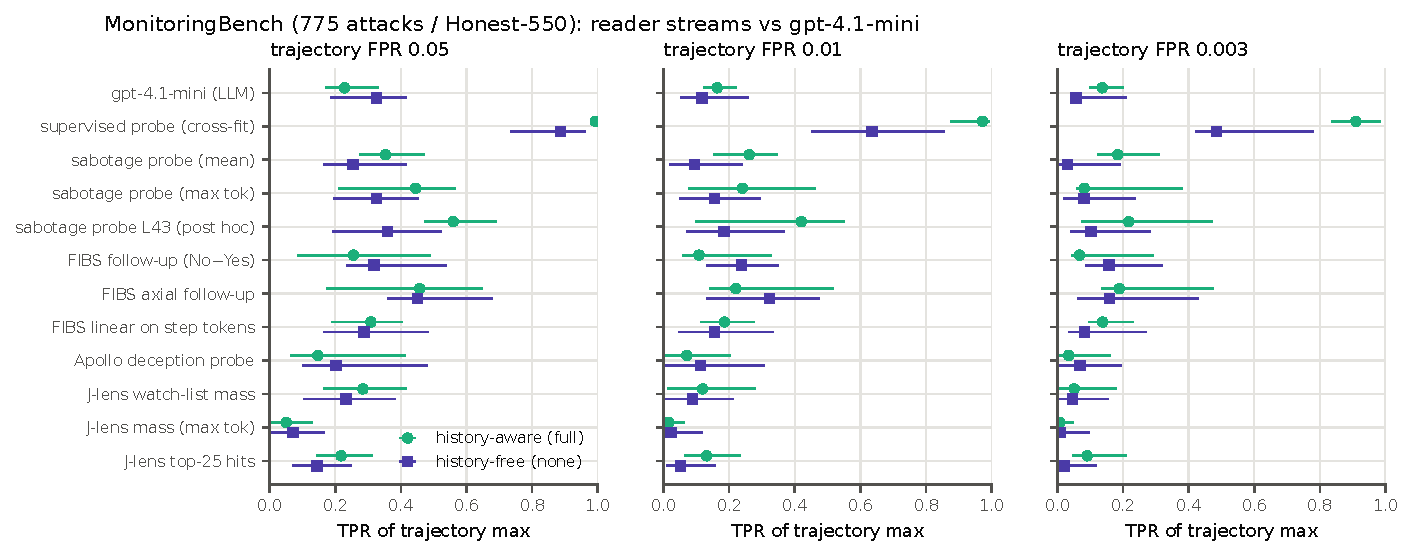
\includegraphics[width=\linewidth]{wb/figures/mb_tpr_max.pdf}
\caption{TPR of the trajectory max at FPR 0.05 / 0.01 / 0.003 with 95\% CIs, per reader stream and the LLM. Green: full reading. Purple: per-step reading (project analysis, nominal FPR).}\label{fig:mbtpr}
\end{figure}

\paragraph{Findings.}
\begin{itemize}
\item \textbf{The per-step FIBS axial follow-up is the one robust win.} It gives TPR 0.34 vs 0.15 for the LLM at 1\% FPR. The gain is $+0.19$ to $+0.21$ across three independent estimates, is equal on opus-4-5 and opus-4-6 attacks, and is unchanged at equal realized FPR. It is the only reader-vs-LLM contrast of 18 that survives Holm. Its AUROC (0.85) is the highest of any non-leaky stream except the post hoc \texttt{sab} L43.
\item \textbf{The full-reading sabotage probe is weakened.} It is nominally $+0.10$ and robust to realized FPR (1.12\% vs 1.42\%), but does not survive Holm ($p=0.22$), and the whole gain is on opus-4-5 attacks ($+0.148$ vs $+0.016$ on opus-4-6): the LLM finds opus-4-6 attacks twice as often, the probe does not. The probe is thus better exactly in the like-for-like comparison (honest and attack agents match), but this is not a family-wise result.
\item \textbf{The full-reading FIBS axial probe runs hot.} At nominal 1\% its realized FPR is 2.05\% (the LLM's is 1.42\%), because some task clusters have heavy honest tails ($\tau=1.64$, \S\ref{sec:ctx}). Its reported $+0.057$ is $\approx+0.06$ at the reader's FPR floor, and that floor is still above the LLM's FPR. Treat this contrast as not shown.
\item \textbf{Generic deception and J-lens readouts lose to the LLM.} The Apollo probe (full) is $-0.09$ [$-0.14$, $-0.01$]. J-lens mass and hits are $-0.03$ to $-0.18$. Max-token J-lens is at chance.
\item \textbf{A post hoc per-layer probe is far better, but unvalidated.} The best single \texttt{sab} layer (L43, chosen on the evaluation set) gives $+0.24$ in full mode at matched FPR. This is a hypothesis for a pre-registered replication, not an estimate.
\end{itemize}


\subsection{Full vs per-step reading}
The same reader under two reading modes plays the role of Idea 1's history-aware vs history-free LLM monitor. The modes favor different signal families:
\begin{itemize}
\item \textbf{Token-level probes prefer full reading.} \texttt{sab} AUROC is 0.79 full vs 0.74 none. Read with context, a step's tokens carry more sabotage signal.
\item \textbf{The follow-up question prefers per-step reading.} FIBS axial AUROC is 0.82 full vs 0.85 none, and TPR at 1\% is 0.25 vs 0.34 (\rf{audit2/repro\_wb\_mb.csv}). In full mode the question is asked after an ever-growing transcript, and honest follow-up scores persist: given one high step, the probability of a second is 0.66--0.77 in full mode vs 0.39--0.47 per step (\rf{wb/mb\_mechanism.csv}). Their honest tails also vary more across task clusters ($\tau$ 1.64 / 2.70 full vs 0.37 / 0.95 none).
\item \textbf{The LLM, like the follow-up probe, separates better per step on AUROC} (0.66 full vs 0.76 none), but its TPRs at 1\% are nearly equal (0.165 vs 0.148).
\item \textbf{Attack structure.} Every stream separates distributed (S4) attacks at least as well as concentrated ones (S1--S3); e.g.\ AUROC on S4 vs S1 is 0.88 vs 0.80 for per-step FIBS axial, 0.81 vs 0.81 for \texttt{sab} full, 0.79 vs 0.73 for the per-step LLM (descriptive; \rf{wb/mb\_subgroups.csv}).
\end{itemize}


\subsection{J-lens watch-list}
\begin{itemize}
\item \textbf{As a monitor the watch-list is weak.} Layer-mean log-mass gives AUROC 0.72 / 0.67 (full / none) and TPR at 1\% below the LLM. Top-25 hit counts give 0.65 / 0.56. Max-token mass is at chance (0.48), which also reflects bf16 noise in max-pooled features.
\item \textbf{Single layers do not help.} AUROC is 0.66 / 0.62 / 0.69 at L27 / L35 / L43 (full) (\rf{wb/mb\_auroc.csv}).
\item \textbf{It is the one signal that helps on MOLE.} There the reader's top-25 hits reach session AUROC 0.96 (max) and 0.98 (mean) (\S\ref{sec:mole}).
\item \textbf{Interpretation.} A trusted reader's J-space reflects the reader's thoughts about the transcript, not the agent's cognition. On BashArena, sysadmin work keeps tokens like \emph{hide}, \emph{monitor} and \emph{secret} high on honest runs as well. This matches the literature note's prediction that a standalone readout is swamped without a baseline.
\end{itemize}

\subsection{(a) Decision rules over probe streams}

\begin{table}[!htbp]\centering\small
\begin{adjustbox}{max width=\linewidth}\begin{tabular}{@{}llccccc@{}}
\toprule
Stream & Mode & 2nd-max & top-3 sum & CUSUM $k{=}0.5$ & CUSUM $k{=}1.5$ & OR(max+CUSUM)\\
\midrule
LLM & full & $+0.029$ [$-0.02$, $+0.10$] & $+0.031$ [$-0.00$, $+0.08$] & $-0.135$ [$-0.18$, $-0.10$] & $+0.018$ [$-0.00$, $+0.05$] & $-0.035$ [$-0.07$, $-0.01$]\\
LLM & none & $+0.041$ [$-0.07$, $+0.11$] & $+0.069$ [$-0.04$, $+0.14$] & $-0.081$ [$-0.19$, $-0.02$] & $-0.002$ [$-0.09$, $+0.05$] & $-0.039$ [$-0.13$, $+0.00$]\\
\texttt{sab} & full & $-0.143$ [$-0.18$, $-0.09$] & $-0.131$ [$-0.17$, $-0.07$] & $-0.207$ [$-0.26$, $-0.12$] & $-0.093$ [$-0.16$, $+0.01$] & $-0.079$ [$-0.13$, $-0.00$]\\
\texttt{sab} & none & $-0.035$ [$-0.09$, $+0.00$] & $-0.044$ [$-0.09$, $-0.01$] & $-0.044$ [$-0.10$, $+0.02$] & $-0.037$ [$-0.10$, $+0.01$] & $-0.021$ [$-0.06$, $+0.02$]\\
FIBS lin.\ follow-up & full & $-0.021$ [$-0.03$, $+0.02$] & $-0.019$ [$-0.04$, $+0.00$] & $-0.002$ [$-0.13$, $+0.05$] & $-0.022$ [$-0.06$, $+0.01$] & $-0.006$ [$-0.10$, $+0.03$]\\
FIBS lin.\ follow-up & none & $-0.124$ [$-0.18$, $-0.05$] & $-0.106$ [$-0.15$, $-0.04$] & $-0.179$ [$-0.25$, $-0.10$] & $-0.182$ [$-0.24$, $-0.08$] & $-0.056$ [$-0.10$, $-0.01$]\\
FIBS axial follow-up & full & $-0.011$ [$-0.05$, $+0.01$] & $-0.024$ [$-0.07$, $-0.00$] & $-0.032$ [$-0.24$, $+0.02$] & $-0.042$ [$-0.11$, $-0.01$] & $-0.001$ [$-0.17$, $+0.04$]\\
FIBS axial follow-up & none & $-0.122$ [$-0.22$, $-0.00$] & $-0.119$ [$-0.19$, $-0.01$] & $-0.246$ [$-0.34$, $-0.13$] & $-0.213$ [$-0.31$, $-0.04$] & $-0.134$ [$-0.21$, $-0.04$]\\
FIBS linear tokens & full & $-0.091$ [$-0.13$, $-0.01$] & $-0.076$ [$-0.11$, $-0.01$] & $-0.133$ [$-0.18$, $-0.05$] & $-0.097$ [$-0.15$, $-0.00$] & $-0.029$ [$-0.08$, $+0.01$]\\
Apollo & none & $-0.045$ [$-0.09$, $+0.02$] & $-0.051$ [$-0.08$, $+0.01$] & $-0.100$ [$-0.15$, $-0.04$] & $-0.064$ [$-0.09$, $+0.02$] & $-0.047$ [$-0.09$, $-0.00$]\\
J-lens mass & none & $-0.026$ [$-0.06$, $+0.03$] & $-0.035$ [$-0.07$, $+0.00$] & $-0.054$ [$-0.10$, $+0.03$] & $-0.061$ [$-0.10$, $-0.01$] & $-0.030$ [$-0.07$, $+0.01$]\\
\bottomrule
\end{tabular}\end{adjustbox}
\caption{TPR difference vs the trajectory max at FPR 0.01 (\rf{wb/tables.md}, \rf{wb/mb\_paired.csv}). No accumulator beats max for any probe stream (only the leaky supervised probe has non-significant positive cells).}\label{tab:acc}
\end{table}

\begin{itemize}
\item \textbf{Max is the right rule on probe streams.} Accumulators are mostly worse, by up to $-0.25$ (CUSUM $k{=}0.5$ on per-step FIBS axial). Idea 1's lesson transfers unchanged: max-type rules first, and CUSUM only with a large reference value.
\item \textbf{Difference-in-differences (none $-$ full) of the CUSUM $k{=}0.5$ gain over max, 1\% FPR.} The sign depends on the probe: \texttt{sab} $+0.163$ [$+0.08$, $+0.22$] (history-free reading favors accumulation, as Idea 1 predicted for LLM monitors); FIBS follow-ups the opposite ($-0.177$ [$-0.25$, $-0.05$] linear, $-0.215$ [$-0.33$, $+0.02$] axial); LLM $+0.054$ [$-0.05$, $+0.12$], n.s. These come from the 10-split analysis and were not in a pre-declared family: exploratory.
\item \textbf{Idea 1's mechanism variables did not flip the ranking anywhere} (descriptive; unit threshold at a 5\% honest step rate, \rf{wb/mb\_mechanism.csv}). Honest spike persistence $P(\ge2\text{ high}\mid\ge1)$ is 0.52 for \texttt{sab} full, 0.77 for FIBS linear follow-up full, 0.33 for the LLM full; the repeat-spike log-LR is 0.37, 0.11 and 0.67. High persistence with low repeat-spike informativeness predicts that accumulation hurts, and it does; even \texttt{sab} none (0.53, 0.26) is outside the regime where accumulation won in Idea 1.
\end{itemize}

\subsection{(b) Per-context probe thresholds}\label{sec:ctx}

\begin{table}[!htbp]\centering\small
\begin{tabular}{@{}lcccc@{}}
\toprule
& \multicolumn{2}{c}{$\tau$ at global 5\% ($p$)} & \multicolumn{2}{c}{context share of honest-max variance}\\
\cmidrule(lr){2-3}\cmidrule(l){4-5}
Stream & full & none & full & none\\
\midrule
LLM (\texttt{gpt-4.1-mini}) & 0.46 (0.16) & 0.00 (1.00) & 0.002 & 0.035\\
\texttt{sab} & 1.21 (0.004) & 0.53 (0.16) & 0.075 & 0.087\\
FIBS linear follow-up & 2.70 ($<$0.001) & 0.95 (0.001) & 0.140 & 0.110\\
FIBS axial follow-up & 1.64 ($<$0.001) & 0.37 (0.27) & 0.107 & 0.068\\
FIBS linear tokens & 0.39 (0.30) & 1.26 ($<$0.001) & 0.029 & 0.048\\
Apollo deception & 3.79 ($<$0.001) & 1.89 (0.001) & 0.036 & 0.103\\
J-lens mass & 0.56 (0.17) & 0.31 (0.37) & 0.030 & 0.020\\
\bottomrule
\end{tabular}
\caption{Between-cluster heterogeneity of honest false-positive rates on 7 MB task clusters: logit-normal $\tau$ at a global 5\% threshold, and the share of honest-max variance explained by cluster (\rf{wb/tables.md}, \rf{wb/context\_heterogeneity.csv}). Per-cluster honest FPRs range up to 0--24.6\% for probes vs 0--12.3\% for the LLM.}\label{tab:tau}
\end{table}

\begin{figure}[!htbp]\centering
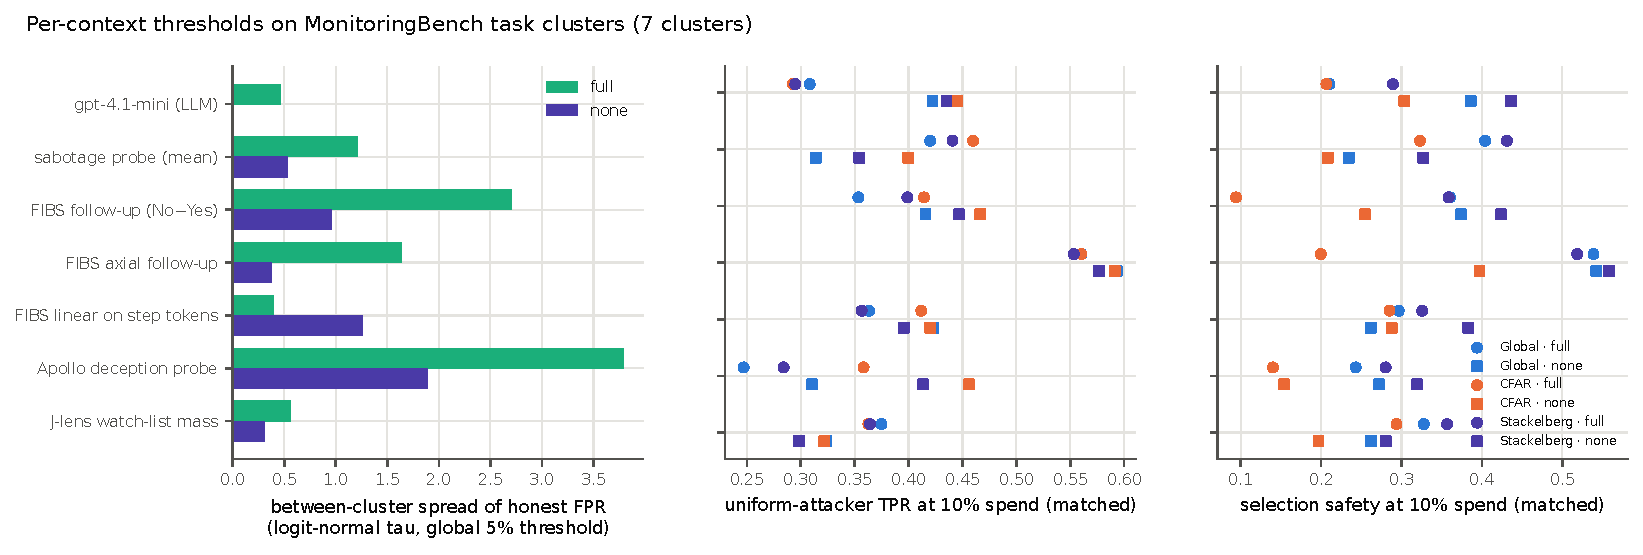
\includegraphics[width=\linewidth]{wb/figures/context_probe_vs_llm.pdf}
\caption{Left: $\tau$ per stream and mode. Middle: uniform-attacker TPR at 10\% spend (spend-matched). Right: safety against an informed context-selecting attacker, for global, CFAR and Stackelberg thresholds.}
\end{figure}

\begin{itemize}
\item \textbf{Probe streams are clearly more context-dependent than the LLM.} $\tau$ is 1.2--3.8 for four probe streams in full mode (all $p\le0.004$) vs 0.46 (n.s.) for the LLM. Cluster share of honest-max variance is 2--14\% vs 0.2--3.5\%. This replicates the context confound reported for Apollo-style probes, and it is the precondition for per-context allocation to matter.
\item \textbf{Allocation at 10\% spend, spend-matched} (CFAR, global and Stackelberg rows matched in $\ge$87\% of replicates; \rf{wb/context\_allocation.csv}). CFAR raises uniform-attacker TPR more for probes than for the LLM, but the only interval excluding 0 is Apollo none, 0.31 $\to$ 0.46 [$+0.01$, $+0.29$], 1 of 14 MB contrasts (\texttt{sab}: full $+0.04$, none $+0.09$, n.s.; LLM $-0.02$ / $+0.02$). CFAR lowers safety against an informed context-selecting attacker (FIBS linear follow-up full: 0.36 $\to$ 0.09, [$-0.46$, $+0.01$]). Stackelberg keeps selection safety within 0.02 of global or above on all 14 MB panels (no interval excludes 0). With 7 clusters most differences are n.s. The 5\% rows (matched in 40--80\% of replicates) and the LinuxArena allocation rows (15--70\%, clamped; audit2 m10) are not used.
\item \textbf{Related correction} (first audit C1, \rf{results/fixes/corrections.csv}). The earlier E5 claim that ``CFAR roughly doubles uniform TPR for probes at 1\%'' is replaced: 1\% spend-matching is not estimable (per-context rules have a realized-spend floor of about 2.5\%), and at equal realized spend CFAR gains $+0.18$ [$+0.08$, $+0.27$] for Apollo full (3.6\%) and $+0.15$ [$+0.03$, $+0.28$] for FIBS linear follow-up full (2.9\%), i.e.\ $1.3$--$1.5\times$, not $2\times$.
\end{itemize}

\subsection{(c) Fusion and triage with the LLM monitor}

\begin{table}[!htbp]\centering\small
\begin{adjustbox}{max width=\linewidth}\begin{tabular}{@{}llcccccc@{}}
\toprule
Probe & Mode & LLM alone & Probe alone & KDE-LLR (traj) & Rank-sum & Cascade 5\% & Cascade 10\%\\
\midrule
\texttt{sab} & full & 0.166 (1.4\%) & 0.258 (1.5\%) & 0.279 (1.0\%) & 0.264 (0.8\%) & 0.306 (1.2\%) & \textbf{0.299} (1.5\%)\\
\texttt{sab} & none & 0.151 (1.3\%) & 0.087 (1.0\%) & 0.201 (1.7\%) & 0.199 (1.2\%) & 0.345 (1.0\%) & 0.280 (1.0\%)\\
FIBS axial f-u & full & 0.166 (1.4\%) & 0.280 (\textbf{2.6\%}) & 0.328 (\textbf{2.8\%}) & 0.293 (1.9\%) & 0.336 (1.8\%) & 0.214 (1.2\%)\\
FIBS axial f-u & none & 0.151 (1.3\%) & \textbf{0.324} (0.9\%) & 0.312 (1.7\%) & 0.314 (2.0\%) & 0.148 (1.3\%) & 0.150 (1.3\%)\\
FIBS lin.\ f-u & full & 0.166 (1.4\%) & 0.137 (2.7\%) & 0.214 (2.8\%) & 0.207 (1.8\%) & 0.319 (1.7\%) & 0.264 (1.4\%)\\
J-lens mass & full & 0.166 (1.4\%) & 0.112 (1.5\%) & 0.221 (2.5\%) & 0.224 (1.3\%) & 0.149 (1.4\%) & 0.162 (1.8\%)\\
\bottomrule
\end{tabular}\end{adjustbox}
\caption{TPR at nominal trajectory FPR 0.01, with \emph{realized} FPR in parentheses (\rf{wb/fusion.csv}). ``Cascade $q$'': the probe flags the top $q$ of honest-calibrated steps, and only those steps go to the LLM, whose score decides. KDE-LLR: a trajectory-level log-likelihood ratio of (probe max, LLM max). Bold FPRs are the A1 problem: realized FPR about $2\times$ nominal.}\label{tab:fusion}
\end{table}

\begin{figure}[!htbp]\centering
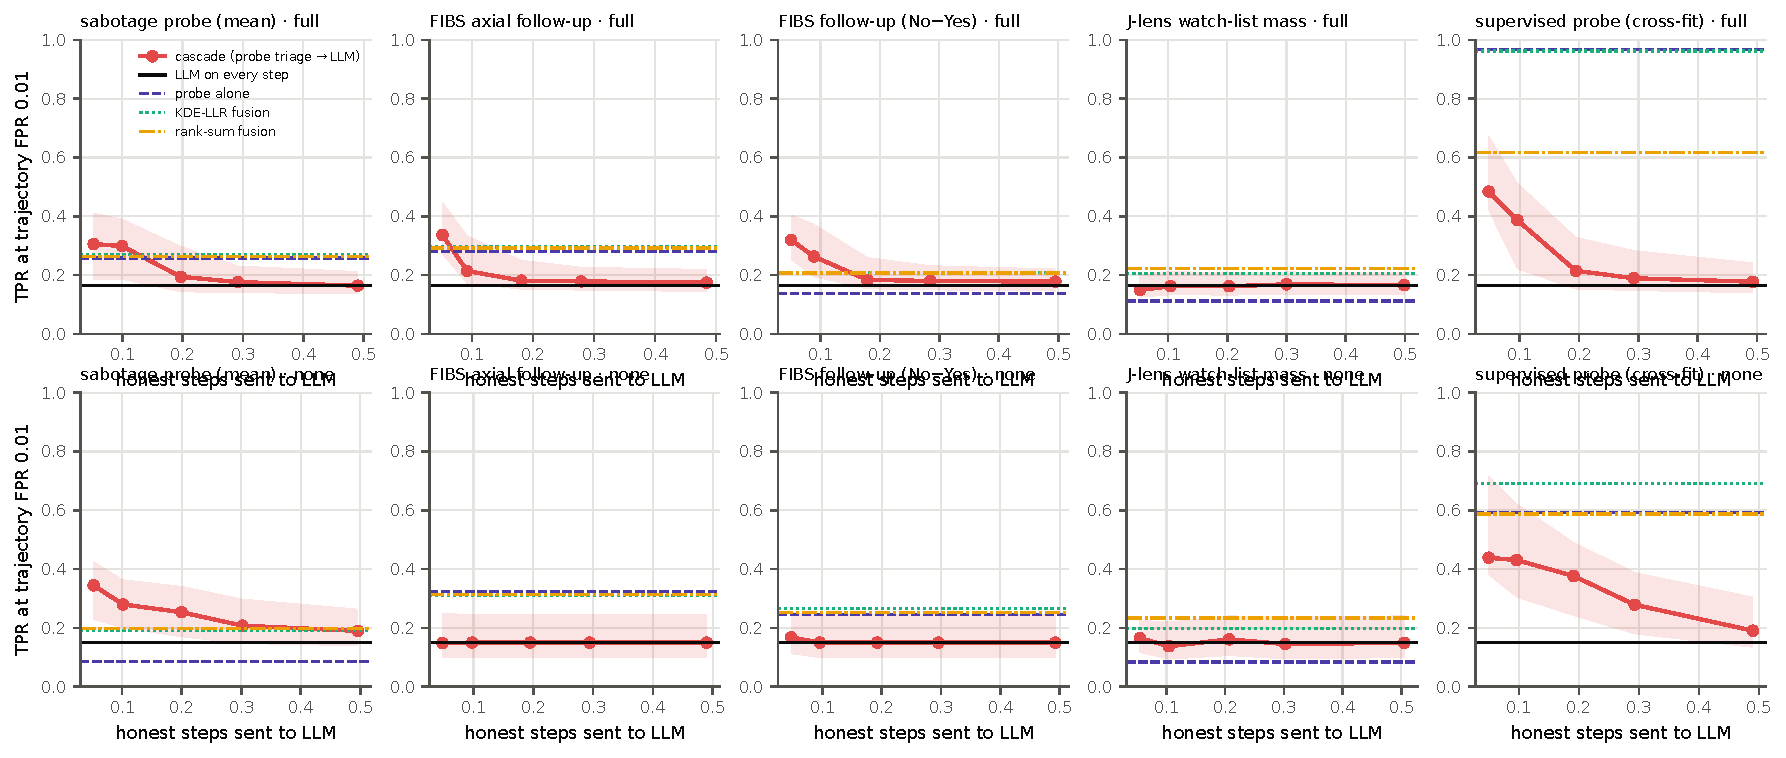
\includegraphics[width=\linewidth]{wb/figures/fusion_cascade.pdf}
\caption{TPR at trajectory FPR 0.01 vs the share of honest steps sent to the LLM (cascade, red), compared with the LLM on every step (black), the probe alone, and KDE-LLR / rank-sum fusion. Top row: full reading. Bottom row: per-step reading.}
\end{figure}

\begin{itemize}
\item \textbf{The \texttt{sab} cascade holds.} Full reading, 10\% of honest-calibrated steps escalated (13.1\% of all steps): TPR 0.298 vs 0.168, $+0.129$ [$+0.07$, $+0.23$], at realized FPR 1.43\% vs 1.81\%, so the cascade does not over-spend (\rf{audit2/repro\_wb\_fusion.csv}). It is a power gain \emph{and} an 87\% cut in LLM calls: the probe removes honest steps the LLM would false-alarm on, so a tighter LLM threshold becomes affordable. Per-step reading gives the same $+0.129$ [$+0.04$, $+0.18$].
\item \textbf{Cascade caveats.} $q=10\%$ was one of 5 levels $\times$ 7 rules $\times$ 5 probes $\times$ 2 modes; $q=5\%$ gives $+0.146$ and $q=20\%$ only $+0.04$ (\rf{audit2/repro\_wb\_fusion.csv}). The gain is $+0.165$ on opus-4-5 attacks vs $+0.067$ on opus-4-6 (\rf{audit2/repro\_wb\_fusion\_strata.csv}).
\item \textbf{FIBS-axial full fusion headlines are weakened (A1).} KDE-LLR's 0.328 ($+0.16$) runs at 2.8\% realized FPR vs 1.4\% for the LLM, so it is not an FPR-matched comparison. The FIBS-axial-full cascade at 5\% (0.336, realized 1.8\%) is closer to matched but shares the problem.
\item \textbf{Per-step FIBS axial needs no LLM.} The probe alone (0.324 at 0.9\% realized FPR) is as good as any fusion. The cascade, in which the LLM decides, falls back to LLM-level TPR.
\item \textbf{Weak probes still help fusion.} J-lens mass in rank-sum fusion is $+0.058$ [$+0.03$, $+0.11$] at 1.3\% realized FPR, although the J-lens alone is below the LLM.
\end{itemize}

\subsection{(d) Probes on detector-aware rewrites}\label{sec:t3}
Idea 3's monitor-aware attacker rewrote MonitoringBench attacks against LLM monitors. Round 2 (pacing arms against \texttt{gpt-4.1}, plus a matched rewrite control) is fully re-analyzable. Round 1's reader streams are lost (A2).

\begin{table}[!htbp]\centering\small
\begin{adjustbox}{max width=\linewidth}\begin{tabular}{@{}lcccccc@{}}
\toprule
& \multicolumn{3}{c}{Detection TPR (FPR 0.01, max)} & \multicolumn{3}{c}{One-shot pace $-$ one-shot control [CI]}\\
\cmidrule(lr){2-4}\cmidrule(l){5-7}
Stream (none) & original & control & pace\_max (r0) & pace\_max & pace\_cusum & pace\_multichart\\
\midrule
\texttt{gpt-4.1} (LLM) & 0.240 & 0.573 & 0.493 & $-0.080$ [$-0.16$, $+0.03$] & $-0.053$ [$-0.11$, $+0.04$] & $-0.093$ [$-0.16$, $-0.01$]\\
FIBS axial follow-up & 0.380 & 0.653 & 0.593 & $-0.060$ [$-0.13$, $+0.03$] & $-0.047$ [$-0.11$, $+0.02$] & $-0.067$ [$-0.14$, $+0.02$]\\
FIBS linear follow-up & 0.227 & 0.513 & 0.500 & $-0.013$ [$-0.10$, $+0.06$] & $-0.027$ [$-0.10$, $+0.06$] & $-0.007$ [$-0.09$, $+0.07$]\\
\texttt{sab} & 0.087 & 0.080 & 0.100 & $+0.020$ [$-0.06$, $+0.09$] & $+0.020$ [$-0.03$, $+0.07$] & $+0.047$ [$+0.00$, $+0.12$]\\
FIBS linear tokens & 0.220 & 0.207 & 0.293 & $+0.087$ [$+0.00$, $+0.16$] & $+0.040$ [$-0.03$, $+0.11$] & $+0.053$ [$-0.02$, $+0.15$]\\
J-lens mass & 0.073 & 0.300 & 0.260 & $-0.040$ [$-0.13$, $+0.08$] & $-0.020$ [$-0.11$, $+0.07$] & $-0.080$ [$-0.15$, $+0.02$]\\
Apollo deception & 0.113 & 0.260 & 0.253 & $-0.007$ [$-0.09$, $+0.07$] & $+0.027$ [$-0.04$, $+0.11$] & $+0.000$ [$-0.08$, $+0.08$]\\
\bottomrule
\end{tabular}\end{adjustbox}
\caption{T3 round 2 (150 base attacks, per-step reading; \rf{wb/tables.md}, \rf{wb/t3\_detection.csv}). ``Control'' is a rewrite with the same rewriter and no pacing instruction. Pacing arms were written against \texttt{gpt-4.1}.}\label{tab:t3}
\end{table}

\begin{figure}[!htbp]\centering
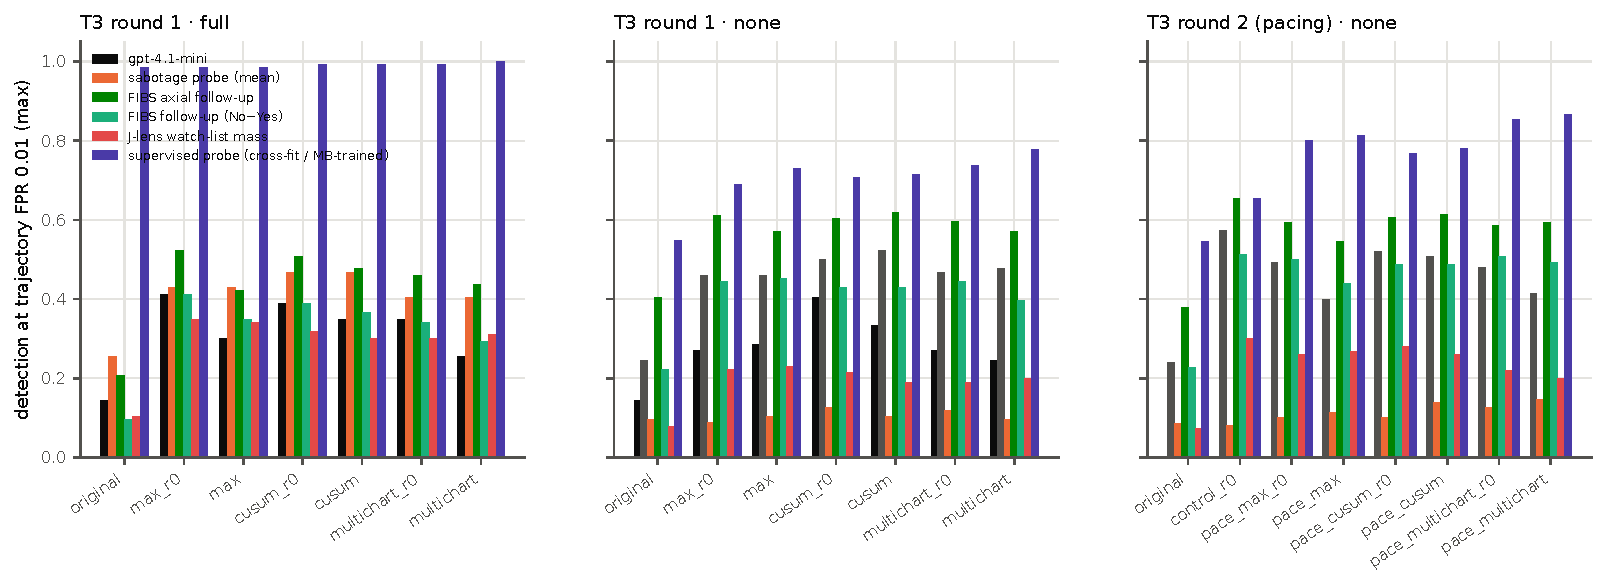
\includegraphics[width=0.92\linewidth]{wb/figures/t3_detection.pdf}
\caption{Detection at trajectory FPR 0.01 (max) on T3 rewrites by arm, for the LLM monitors and reader streams. Round 1 (left, middle) is not reproducible from stored data (A2). Round 2 (right) is intact.}
\end{figure}

\begin{itemize}
\item \textbf{The rewrite artifact is monitor-type specific.} The control rewrite roughly doubles detection by \texttt{gpt-4.1} (0.24 $\to$ 0.57) and the follow-up probes (FIBS axial 0.38 $\to$ 0.65), but leaves token-level probes unchanged (\texttt{sab} 0.087 $\to$ 0.080; FIBS tokens 0.22 $\to$ 0.21). The rewrites condense attacks and carry fabricated tool outputs (first audit M5); monitors that \emph{ask a question about the transcript} react to that, probes on the action tokens do not.
\item \textbf{Pacing written against \texttt{gpt-4.1} transfers partly to the follow-up probe, not to token probes.} One-shot pacing vs one-shot control is $-0.05$ to $-0.09$ for \texttt{gpt-4.1} and $-0.05$ to $-0.07$ (n.s.) for FIBS axial, but $+0.02$ to $+0.09$ for \texttt{sab} and FIBS tokens. No contrast is Holm-corrected. Only \texttt{gpt-4.1} pace\_multichart has an interval excluding 0 in the evasion direction.
\item \textbf{Why the token probes do not see the artifact.} On the E5 panel (first audit, M5) the same pattern appears as an AUROC confound. Refined variants of the same base attacks score higher than their originals for FIBS linear follow-up full ($+0.20$ [$+0.11$, $+0.30$]) and Apollo full ($+0.31$). They do not score higher for \texttt{sab} max-token ($-0.07$ [$-0.16$, $+0.01$]). On the 33 unrewritten originals the \texttt{sab} probes have the highest AUROC (0.81--0.83, vs \texttt{gpt-4.1} 0.77) (\rf{fixes/corrections.csv}).
\item \textbf{Scope.} Every arm is an LLM-monitor-aware \emph{prompted} rewrite. None is a probe-aware or trained evader, so this says nothing about robustness to the attacks in \S\ref{sec:prior}.
\end{itemize}

\subsection{LinuxArena}
\begin{figure}[!htbp]\centering
\begin{minipage}[c]{0.42\linewidth}\centering
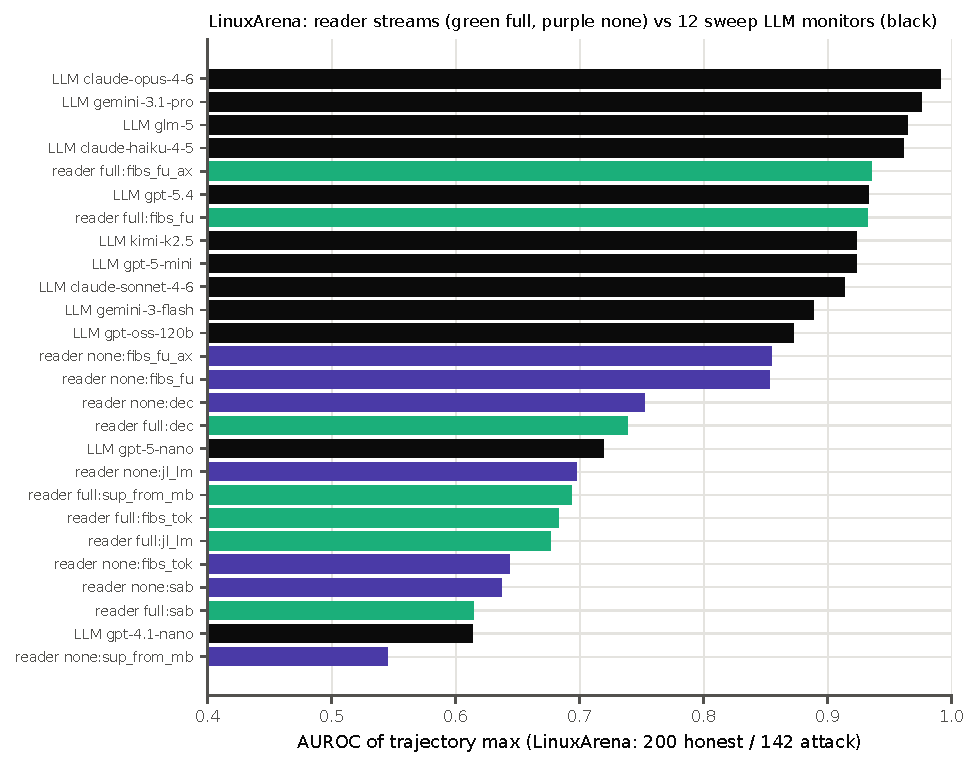
\includegraphics[width=\linewidth]{wb/figures/la_auroc.pdf}
\end{minipage}\hfill
\begin{minipage}[c]{0.55\linewidth}\centering\scriptsize
\setlength{\tabcolsep}{3pt}
\begin{adjustbox}{max width=\linewidth}\begin{tabular}{@{}lccc@{}}
\toprule
Monitor & AUROC & TPR@0.05 & TPR@0.01\\
\midrule
LLM \texttt{claude-opus-4-6} & 0.991 & 0.943 [0.90, 0.99] & 0.923 [0.79, 0.97]\\
LLM \texttt{gemini-3.1-pro} & 0.976 & 0.934 [0.87, 0.98] & 0.902 [0.27, 0.95]\\
Reader FIBS axial f-u (full) & 0.936 & 0.825 [0.75, 0.89] & 0.756 [0.56, 0.86]\\
LLM \texttt{gpt-5.4} & 0.933 & 0.702 [0.58, 0.86] & 0.568 [0.37, 0.70]\\
Reader FIBS linear f-u (full) & 0.932 & 0.784 [0.69, 0.88] & 0.713 [0.57, 0.82]\\
LLM \texttt{claude-sonnet-4-6} & 0.913 & 0.707 [0.62, 0.83] & 0.645 [0.52, 0.75]\\
Reader FIBS axial f-u (none) & 0.854 & 0.446 [0.13, 0.66] & 0.167 [0.04, 0.52]\\
Reader J-lens hits (full) & 0.754 & 0.419 [0.28, 0.57] & 0.297 [0.19, 0.48]\\
Reader \texttt{sab} (full) & 0.615 & 0.262 [0.14, 0.35] & 0.159 [0.07, 0.30]\\
LLM \texttt{gpt-4.1-nano} & 0.613 & 0.193 [0.11, 0.29] & 0.120 [0.04, 0.22]\\
\bottomrule
\end{tabular}\end{adjustbox}
\end{minipage}
\caption{LinuxArena (200 honest, 142 attacks), trajectory max. Left: AUROC of reader streams (green full, purple per-step) vs 12 LLM monitors (black) on the same trajectories (\rf{wb/la\_auroc.csv}). Right: excerpt with marginal 95\% CIs (\rf{wb/tables.md}). The reader score files behind these numbers are lost (A2).}
\end{figure}

\begin{itemize}
\item \textbf{FIBS follow-up probes in full reading are comparable to mid-tier frontier monitors.} AUROC is 0.93--0.94, against \texttt{gpt-5.4} at 0.933 and \texttt{sonnet-4-6} at 0.913. They are below \texttt{opus-4-6} and \texttt{gemini-3.1-pro}.
\item \textbf{The ranking is weakened (audit2 m3).} Only marginal CIs exist and they overlap ([0.56, 0.86] vs [0.37, 0.70] for \texttt{gpt-5.4}); the 1\% threshold is the top of about 100 calibration honest runs; no paired test was run, and none can be run now (A2).
\item \textbf{Mode reversal.} Unlike MB, full reading beats per-step reading here (0.94 vs 0.85).
\item \textbf{The sabotage probe and J-lens are weak} (AUROC 0.62--0.75). The \texttt{sab} contrast pairs were generated from generic objectives, and LinuxArena's side tasks are more diverse.
\end{itemize}

\subsection{Stage 2: policy vs reader activations on MOLE}\label{sec:mole}
\begin{itemize}
\item \textbf{Policy arm.} Qwen3.6-27B, the model that generated MOLE's \texttt{qwen36\_27b} single-day sessions, reads its own sessions in its chat format, including the system prompt. That prompt states the insider objective. Reasoning tokens and tool schemas are not in the release.
\item \textbf{Reader arm.} Qwen3.5-27B in the monitor framing, without the system prompt.
\item \textbf{Probes.} \texttt{sab} was re-trained on each model's own activations of the same contrast pairs (CV AUROC 0.97 for both; \rf{EXPERIMENT\_LOG.md}). The FIBS 3.5 linear probe is applied to Qwen3.6 as a transfer.
\end{itemize}

\begin{table}[!htbp]\centering\small
\begin{adjustbox}{max width=\linewidth}\begin{tabular}{@{}lcccc@{}}
\toprule
& \multicolumn{2}{c}{Policy (Qwen3.6-27B)} & \multicolumn{2}{c}{Reader (Qwen3.5-27B)}\\
\cmidrule(lr){2-3}\cmidrule(l){4-5}
Stream & max over turns & mean over turns & max over turns & mean over turns\\
\midrule
\texttt{sab} (layer mean) & 0.839 [0.80, 0.88] & 0.954 [0.94, 0.97] & 0.863 [0.83, 0.89] & 0.955 [0.94, 0.97]\\
\texttt{sab} L43 (post hoc) & 0.899 [0.87, 0.93] & 0.978 [0.96, 0.99] & 0.938 [0.92, 0.96] & 0.982 [0.97, 0.99]\\
FIBS linear on tokens & 0.816 [0.78, 0.86] & \textbf{0.982} [0.97, 0.99] & 0.620 [0.57, 0.67] & 0.742 [0.70, 0.79]\\
J-lens mass & 0.683 [0.64, 0.73] & 0.764 [0.72, 0.80] & 0.752 [0.71, 0.80] & 0.829 [0.79, 0.87]\\
J-lens top-25 hits & 0.800 [0.76, 0.84] & 0.925 [0.90, 0.95] & 0.956 [0.94, 0.97] & \textbf{0.984} [0.97, 0.99]\\
\bottomrule
\end{tabular}\end{adjustbox}
\caption{Session AUROC, 233 insider vs 200 random benign sessions (\rf{wb/mole\_policy\_vs\_reader.csv}). TPR at 1\% FPR for \texttt{sab} mean: policy 0.71, reader 0.74.}
\end{table}


\begin{itemize}
\item \textbf{Policy activations do not beat the reader on the main probe} (\texttt{sab}: 0.84 / 0.95 vs 0.86 / 0.96).
\item \textbf{The one stream where the policy wins is suspect.} FIBS on tokens gives 0.98 vs 0.74 (mean), but this is also the stream that could key on the in-context insider instruction, which only the policy sees.
\item \textbf{The reader's J-lens hit count is the best stream of either arm} (0.96 / 0.98).
\item \textbf{The split cannot answer the policy-vs-reader question cleanly.} There is no LLM baseline for it; benign sessions are a random sample whose account and role mix is not matched to the insiders, so session-type differences may inflate every AUROC; and the policy sees a system prompt that names the objective.
\end{itemize}

\section{What holds, what is weakened, what is dropped}
Table~\ref{tab:ledger} lists every headline claim with its verdict after the first audit (\rf{results/fixes/}) and the second audit (\rf{results/audit2/}).

\begin{table}[!htbp]\centering\footnotesize
\begin{tabularx}{\linewidth}{@{}>{\raggedright\arraybackslash}p{5.0cm}>{\raggedright\arraybackslash}p{2.1cm}>{\raggedright\arraybackslash}X@{}}
\toprule
Claim & Verdict & Basis\\
\midrule
Per-step FIBS axial follow-up beats \texttt{gpt-4.1-mini} at 1\% FPR & \textbf{holds} & $+0.206$ / $+0.194$ / $+0.185$ (10 / 40 / 200 splits); $+0.183$ at equal realized FPR; both agent models; only Holm survivor of 18 (audit2 m1, m2)\\
\texttt{sab} cascade (10\%) beats the LLM with 87\% fewer calls & \textbf{holds} & 0.298 vs 0.168, $+0.129$ [$+0.07$, $+0.23$] at realized FPR 1.43\% vs 1.81\% (audit2 m4); $q$ chosen among 5; larger on opus-4-5\\
No accumulation rule beats max on probe streams & \textbf{holds} & Table~\ref{tab:acc}; consistent with Idea 1\\
Probe streams are more context-heterogeneous than LLM streams & \textbf{holds} & honest-only statistic, unaffected by matching issues (first audit M5 row)\\
Full-reading \texttt{sab} beats the LLM ($+0.10$) & weakened & Holm $p=0.22$; $+0.148$ on opus-4-5 vs $+0.016$ on opus-4-6 (audit2 m2)\\
Full-reading FIBS axial beats the LLM ($+0.057$) & weakened / not shown & realized FPR 2.05\% vs 1.42\%; floor 1.58\%; $+0.059$ at the floor (audit2 A1)\\
FIBS-axial-full fusion (KDE-LLR 0.328, $+0.16$) & weakened & realized FPR 2.8\% vs 1.4\% (audit2 A1)\\
LinuxArena: FIBS follow-up above \texttt{gpt-5.4} and four others & weakened, unverifiable & no paired test; score files lost (audit2 m3, A2)\\
T3 round-1 reader detection rows & unverifiable & score files lost (A2); round 2 intact and consistent\\
CFAR on probes ``roughly doubles'' uniform TPR (E5, 1\%) & dropped / replaced & 1\% matching not estimable; $1.3$--$1.5\times$ at equal realized spend (first audit C1)\\
\texttt{sab} L43 ($+0.24$) & exploratory only & selected on the evaluation set\\
DiD of CUSUM gain (\texttt{sab} $+0.16$; FIBS $-0.18$) & exploratory & 10 splits, not in a declared family\\
MOLE: policy activations add nothing over the reader & holds, weak design & unmatched benign sessions, no LLM baseline, objective in the policy's context\\
\bottomrule
\end{tabularx}
\caption{Claim ledger after both audits (\rf{results/audit2/corrections.csv}, \rf{results/audit2/issues.csv}, \rf{results/fixes/corrections.csv}).}
\label{tab:ledger}
\end{table}

\section{Interpretation}
\begin{enumerate}
\item \textbf{A trusted reader buys some power, not only cost savings.} The literature note expected ``white-box adds cost savings, not power, for a trusted reader''. One off-the-shelf probe (FIBS axial) on a per-step follow-up question beats a cheap LLM monitor by about 0.19 TPR at 1\% FPR with no task-specific training. The comparator is weak (\texttt{gpt-4.1-mini}, AUROC 0.66--0.76), so ``beats a cheap LLM monitor'' is the right scope; on LinuxArena the strongest frontier monitors remain ahead.
\item \textbf{The probe's best use with an LLM is triage.} The \texttt{sab} cascade gains about 0.13 TPR \emph{and} removes about 87\% of LLM calls, the shape of the published GDM and Anthropic misuse cascades\uv, here at matched trajectory FPR for multi-step sabotage.
\item \textbf{Probe streams need context-aware calibration.} Their between-task heterogeneity is much larger ($\tau$ 1.2--3.8 for four probe streams vs 0.46 for the LLM), and the one audit failure (A1) is exactly a probe threshold that did not transfer across tasks. Per-context allocation helps only modestly at matched spend, and CFAR is exploitable by a context-selecting attacker; Stackelberg is the safe default, as in Idea 2.
\item \textbf{The decision layer transfers unchanged.} Max is the right trajectory rule on every probe stream.
\item \textbf{Token-level probes and question-based monitors fail differently.} Rewriting artifacts move LLM monitors and follow-up probes but not token probes, an argument for combining the two kinds. It is not robustness evidence: no attacker here knew about the probes.
\end{enumerate}

\section{Limitations}
\begin{itemize}
\item \textbf{One reader, one MB comparator} (\texttt{gpt-4.1-mini}); no frontier LLM monitor was run on MB.
\item \textbf{Statistical power.} 550 honest runs put a 1\% trajectory FPR on about 5 false alarms per calibration half; the project analysis used 10 splits; 7 MB clusters are too few for per-context significance.
\item \textbf{Off-policy reading.} The reader reads Opus-authored text, the regime where intent probes generalize worst, and shares an LLM monitor's threat model (it sees only text).
\item \textbf{Label-correlated agent model.} Honest runs are all opus-4-5; like-for-like results are reported, but surface features (truncation, reasoning visibility) remain label-correlated (first audit m8).
\item \textbf{Lost data} (LinuxArena, T3-r1 reader streams; A2), \textbf{no adaptive white-box attacker} (every robustness concern in \S\ref{sec:prior} stands untested), and \textbf{bf16 noise} in max-pooled features (up to 2 SD for single steps).
\end{itemize}

\section{Recommended next steps}
\begin{enumerate}
\item \textbf{Preregister and Holm-control a small confirmatory family} on a fresh split: (i) per-step FIBS axial vs the LLM; (ii) the \texttt{sab} cascade at a pre-declared $q$; (iii) \texttt{sab} L43 in full reading, replicating the post hoc layer. Use $\ge$100 grouped splits, report realized FPR next to every TPR, and compare at equal realized FPR.
\item \textbf{Regenerate the lost score files.} Re-read LinuxArena (342 trajectories) and T3 round 1 (509 attacks) in both modes (about 1--2 H200-hours), then run the missing paired LinuxArena contrasts. Guard the sync so it never overwrites a non-empty local file with an empty one.
\item \textbf{Calibrate the full-reading FIBS axial threshold per cluster} (Stackelberg or partially pooled) and re-state the full-mode fusions at matched realized FPR.
\item \textbf{Build a proper policy-activation arm}: matched benign sessions (same accounts, roles and days), an LLM baseline on the same split, an arm with the objective removed from the system prompt; better, fresh open-policy rollouts (e.g.\ Qwen3.6-27B on BashArena) with reasoning retained, so both arms see identical text.
\item \textbf{Add a strong LLM comparator on MB} (\texttt{gpt-4.1} or a frontier monitor on the same 1{,}325 trajectories) to test whether the FIBS-axial gain survives against a non-trivial monitor.
\item \textbf{Run a probe-aware attacker}: first prompted (``a white-box probe on a trusted model reads your actions'') against a strong LLM monitor; then, if stage 1 holds, a trained RL-Obfuscation-style evader.
\item \textbf{Contact FAR.AI} for FIBS's on-policy BashArena and SHADE step streams; our aggregation, per-context and cascade analyses would run on them unchanged.
\end{enumerate}

\section*{Cost and reproduction}
GPU $\approx$\$70 (two on-demand H200 pods, about 7.0 h and 5.8 h at \$5.29/h, plus \$2.1 of earlier setup; about 1{,}000 tokens/s per reader process with per-step follow-ups); OpenRouter \$2.95 (contrast pairs); second audit \$0. Code: \texttt{tracks/wb\_whitebox/} (reader and analyses) and \texttt{tracks/audit2/}. Results: \texttt{results/wb/} (tables.md, CSVs, figures), \texttt{results/audit2/}, errata \texttt{results/fixes/corrections.csv}. Score streams: \texttt{data/processed/whitebox/scores/} (MB, T3 r2 and MOLE intact; LinuxArena and T3 r1 empty). Log: \texttt{EXPERIMENT\_LOG.md} (2026-10-21/22). Repository: \url{https://github.com/gregkocher/agent-monitor-detection} (private).
\end{document}
